\documentclass[sigconf]{acmart}

\usepackage{booktabs} % For formal tables
\usepackage[outdir=../build/]{epstopdf}


% Copyright
%\setcopyright{none}
%\setcopyright{acmcopyright}
%\setcopyright{acmlicensed}
\setcopyright{rightsretained}
%\setcopyright{usgov}
%\setcopyright{usgovmixed}
%\setcopyright{cagov}
%\setcopyright{cagovmixed}


% DOI
\acmDOI{10.1145/nnnnnnn.nnnnnnn}

% ISBN
\acmISBN{978-x-xxxx-xxxx-x/YY/MM}


%Conference
\acmConference[GECCO '18]{the Genetic and Evolutionary Computation
Conference 2018}{July 15--19, 2018}{Kyoto, Japan}
\acmYear{2018}
\copyrightyear{2018}


\acmArticle{4}
\acmPrice{15.00}

% These commands are optional
%\acmBooktitle{Transactions of the ACM Woodstock conference}
\editor{Jennifer B. Sartor}
\editor{Theo D'Hondt}
\editor{Wolfgang De Meuter}


\begin{document}
\title{SIG Proceedings Paper in LaTeX Format}
\titlenote{Produces the permission block, and
  copyright information}
\subtitle{Extended Abstract}
\subtitlenote{The full version of the author's guide is available as
  \texttt{acmart.pdf} document}


%\author{Ben Trovato}
%\authornote{Dr.~Trovato insisted his name be first.}
%\orcid{1234-5678-9012}
%\affiliation{%
%  \institution{Institute for Clarity in Documentation}
%  \streetaddress{P.O. Box 1212}
%  \city{Dublin} 
%  \state{Ohio} 
%  \postcode{43017-6221}
%}
%\email{trovato@corporation.com}
%
%\author{G.K.M. Tobin}
%\authornote{The secretary disavows any knowledge of this author's actions.}
%\affiliation{%
%  \institution{Institute for Clarity in Documentation}
%  \streetaddress{P.O. Box 1212}
%  \city{Dublin} 
%  \state{Ohio} 
%  \postcode{43017-6221}
%}
%\email{webmaster@marysville-ohio.com}
%
%\author{Lars Th{\o}rv{\"a}ld}
%\authornote{This author is the
%  one who did all the really hard work.}
%\affiliation{%
%  \institution{The Th{\o}rv{\"a}ld Group}
%  \streetaddress{1 Th{\o}rv{\"a}ld Circle}
%  \city{Hekla} 
%  \country{Iceland}}
%\email{larst@affiliation.org}
%
%\author{Valerie B\'eranger}
%\affiliation{%
%  \institution{Inria Paris-Rocquencourt}
%  \city{Rocquencourt}
%  \country{France}
%}
%\author{Aparna Patel} 
%\affiliation{%
% \institution{Rajiv Gandhi University}
% \streetaddress{Rono-Hills}
% \city{Doimukh} 
% \state{Arunachal Pradesh}
% \country{India}}
%\author{Huifen Chan}
%\affiliation{%
%  \institution{Tsinghua University}
%  \streetaddress{30 Shuangqing Rd}
%  \city{Haidian Qu} 
%  \state{Beijing Shi}
%  \country{China}
%}
%
%\author{Charles Palmer}
%\affiliation{%
%  \institution{Palmer Research Laboratories}
%  \streetaddress{8600 Datapoint Drive}
%  \city{San Antonio}
%  \state{Texas} 
%  \postcode{78229}}
%\email{cpalmer@prl.com}
%
%\author{John Smith}
%\affiliation{\institution{The Th{\o}rv{\"a}ld Group}}
%\email{jsmith@affiliation.org}
%
%\author{Julius P.~Kumquat}
%\affiliation{\institution{The Kumquat Consortium}}
%\email{jpkumquat@consortium.net}

% The default list of authors is too long for headers.
%\renewcommand{\shortauthors}{B. Trovato et al.}


\begin{abstract}
    In genetic algorithms, the importance of the basis for representation has been well known.
In this paper, we emprirically studied the effect of a \textit{good basis} in binary representation, where a \textit{good basis} means a basis that can improve the serch performance of search algorithms.
A complicated problem space may be transformed into a linearly-separable one via a change of basis.
We had experiments on the one-max problem to clearly see the effect of basis change on search performance.
From these experiments, we could see that search performance is not so good with badly-designed genetic operators.
On the other hand, finding a good basis from all the bases may not be practical, because it takes time as $ O(2^{n^2}) $, where $ n $ is the length of a chromosome.
However, we used a genetic algorithm to find a good basis, to correctly inverstigate how a good basis affects the problem space.
We also conducted experiments on the $ NK $-landscape model as a representative computationally hard problem.
Experimental results showed that changing basis by the presented genetic algorithm always leads better search performance on the $ NK $-landscape model.

\end{abstract}

%
% The code below should be generated by the tool at
% http://dl.acm.org/ccs.cfm
% Please copy and paste the code instead of the example below. 
%
\begin{CCSXML}
<ccs2012>
 <concept>
  <concept_id>10010520.10010553.10010562</concept_id>
  <concept_desc>Computer systems organization~Embedded systems</concept_desc>
  <concept_significance>500</concept_significance>
 </concept>
 <concept>
  <concept_id>10010520.10010575.10010755</concept_id>
  <concept_desc>Computer systems organization~Redundancy</concept_desc>
  <concept_significance>300</concept_significance>
 </concept>
 <concept>
  <concept_id>10010520.10010553.10010554</concept_id>
  <concept_desc>Computer systems organization~Robotics</concept_desc>
  <concept_significance>100</concept_significance>
 </concept>
 <concept>
  <concept_id>10003033.10003083.10003095</concept_id>
  <concept_desc>Networks~Network reliability</concept_desc>
  <concept_significance>100</concept_significance>
 </concept>
</ccs2012>  
\end{CCSXML}

\ccsdesc[500]{Computer systems organization~Embedded systems}
\ccsdesc[300]{Computer systems organization~Redundancy}
\ccsdesc{Computer systems organization~Robotics}
\ccsdesc[100]{Networks~Network reliability}


\keywords{ACM proceedings, \LaTeX, text tagging}


\maketitle

\section{Introduction}
A matrix $ A $ is called \textit{binary} if $ A \in M_{n \times n}(\Z_2) $~\cite{kim2008two}.
Binary matrices have been widely used to deal with the adjacency of a graph~\cite{anderson1998turning, biggs1993algebraic,brualdi1991combinatorial, kim2005new}.
In particular,
Anderson and Feil~\cite{anderson1998turning} transformed the \textit{light bulb puzzle} into the problem of solving a linear system $ A\mathbf{x} = \mathbf{b} $ from its graph structure,
where $ A \in M_{n \times n } $ and $ \mathbf{x},\, \mathbf{b} \in \Z_2^n $.
Then, the solution is obtained by computing the inverse of $ A $, that is, $ \mathbf{x} = A^{-1} \mathbf{b} $.
Binary matrices are also useful in dealing with the \textit{cut/cycle} subspace of a graph, which is a vector space over $ \Z_2 $~\cite{biggs1993algebraic,yoon2011note}.
They can also be used to represent a change of basis of a vector space over $ \Z_2 $ in combinatorial problems~\cite{kim2008linear,kim2008effect}.
A change of basis plays an important role in the performance of evolutionary algorithms~\cite{kim2008effect,hwang2006multi,kim2003problem,seo2012spanning,wyatt2003finding}.

In this paper,
we investigate how to find a good basis in the space of nonsingular binary matrices, $ GL_n(\Z_2)$.
Table~\ref{tab:space} shows the sizes of spaces according to small $ n $.
The size of $ \Z_2^n $ and $ GL_n(\Z_2) $ are $ 2^n $ and $ O(2^{n^2}) $, respectively.
We used a genetic algorithm to find a good basis affecting the problem space.

The paper is organized as follows.
In Section \ref{section:ccm_intro}, we introduce how a nonsingular binary matrix changes the basis.
We design a genetic algorithm to find a good basis in Section~\ref{section:ga_ccm}.
In Section ~\ref{section:encoding}, we introduce the encoding for change of coordinate matrix, $ GL_n(\Z_2) $.
We introduce the elementary matrix of $ M_{n \times n}(\Z_2) $,
to represent a nonsingular binary matrix as a product of elementary matrices.
This induces the representation by a variable-length linear string~\cite{yoon2014mathematical}, and the representation is not unique.
It is not so easy to know how many equivalent representations exist for a nonsingular binary matrix.
We analyze the nontrivial equivalence that has not existed before.
In Section~\ref{section:genetic_operator}, we propose genetic operators for variable-length linear string with elementary matrices, and in Section~\ref{section:experiments} we analyze the experimental results.
We give discussion including future work in Section ~\ref{section:conclusions}.








\section{Change of Coordinate Matrix in \texorpdfstring{$ GL_n(\Z_2) $}{GL\_{}n(Z\_{}2)}} \label{section:ccm_intro}

\subsection{Change of Coordinate Matrix}
We introduce some notations and theorems for change of basis in $ GL_n(\Z_2) $ \cite{friedberglinear}.

\begin{theorem} \label{theorem:ccm}
Let $ \B $ and $ \B^\prime $ be two ordered bases for a finite-dimensional vector space $ V $,
and let $ Q = \left[ \1_V \right]_{\B}^{\B^\prime} $. Then
\begin{enumerate}
    \item $ Q $ is invertible.
    \item For any $\, v \in V,\, \left[ v \right]_{\B^\prime} = Q \left[ v \right]_{\B} $.
\end{enumerate}
\end{theorem}

Observe that if $ \B = \left\{ u_1, u_2, \ldots, u_n \right\} $
and $ \B^\prime = \left\{ u_1^\prime, u_2^\prime, \ldots, u_n^\prime \right\} $,
then
\[ u_j = \sum_{i=1}^{n} { Q_{ij} u_i^\prime } \] for $ j = 1, 2, \ldots, n $,
which implies the $ j $-th column of $ Q $ is $ [ u_j ]_{\B^\prime} $ and $ Q $ changes $ \B $-coordinates into $ \B^\prime $-coordinates.

\begin{Definition}
The matrix $ Q = \left[ \1_V \right]_{\B}^{\B^\prime} $
defined in Theorem~\ref{theorem:ccm} is called a \text{\normalfont change of coordinate matrix}.
\end{Definition}

In this paper, we consider a problem based on binary representation.
This means that each solution of the problem belongs to the vector space $ \Z_2^n $,
where $ n $ is the problem size.
The following is an example of the one-max problem applying a change of basis.
Here, the one-max problem is to find a vector with a value of $ 1 $ for each element.

Let $ \B $ and $ \B^\prime $ be two ordered bases for the one-max problem with problem size of $ 3 $.
The baese are as follows:
\begin{align*}
    \B         &= \{ (1,0,0), (0,1,0), (0,0,1) \} = \{ e_1,        e_2,        e_3 \}, \\
    \B^\prime  &= \{ (1,0,1), (0,0,1), (0,1,0) \} = \{ e_1^\prime, e_2^\prime, e_3^\prime \}.
\end{align*}
Note that
\begin{align*}
    \1_V(e_1) &= 1 \cdot e_1^\prime + 1 \cdot e_2^\prime + 0 \cdot e_3^\prime, \\
    \1_V(e_2) &= 0 \cdot e_1^\prime + 0 \cdot e_2^\prime + 1 \cdot e_3^\prime, \text{ and} \\
    \1_V(e_3) &= 0 \cdot e_1^\prime + 1 \cdot e_2^\prime + 0 \cdot e_3^\prime.
\end{align*}
Hence, matrix $ Q = \left[ \1_V \right]_{\B}^{\B^\prime} $ as follows:
\[
    Q = \begin{pmatrix}
        1 & 0 & 0 \\
        1 & 0 & 1 \\
        0 & 1 & 0
    \end{pmatrix}
    \begin{matrix}
        \vphantom{0} \\
        \vphantom{1} \\
        \vphantom{0}.
    \end{matrix}
\]
The elements of the one-max problem based on the standard basis are shown in Table~\ref{tab:one-max} for each element.

\begin{table}[H]
  \caption{All the solutions in the one-max problem according to basis}
  \label{tab:one-max}
  \begin{tabularx}{0.45\textwidth}{ *{1}{>{\centering\hsize=0.25\hsize}X} *{2}{Y}}
    \toprule
    Fitness & Elements based on $ \B $ & Elements based on $ \B^\prime $\\
    \midrule
    $ 3 $                  &  $ (1,1,1) $  &  $ (1,0,1) $ \\ \hline
    \multirow{3}{*}{$ 2 $} &  $ (1,1,0) $  &  $ (1,1,1) $ \\
                           &  $ (1,0,1) $  &  $ (1,0,0) $ \\
                           &  $ (0,1,1) $  &  $ (0,1,1) $ \\ 
    \midrule
    \multirow{3}{*}{$ 1 $} &  $ (1,0,0) $  &  $ (1,1,0) $ \\
                           &  $ (0,1,0) $  &  $ (0,1,0) $ \\
                           &  $ (0,0,1) $  &  $ (0,0,1) $ \\ \hline
    $ 0 $                  &  $ (0,0,0) $  &  $ (0,0,0) $ \\
  \bottomrule
\end{tabularx}
\end{table}

We know that the element of $ GL_n(\Z_2) $ is the medium that transforms the vector or $ \Z_2^n $ to the coordinate of a certain basis in the binary representation.
To investigate all the bases, the basis as many as the number of $ \left| GL_n(\Z_2) \right| $ should be investigated.
Consider the following equation.
\[ GL_n(\Z_2) = \prod\limits_{k=0}^{n-1} \left( 2^n - 2^k \right) \in O(2^{n^2}). \]
It may be meaningful to investigate all the bases in $ GL_n(\Z_2) $, but it takes $ O(2^{n^2}) $ time, which is too time consuming.
Therefore, we conduct an experimental research on the distribution and importance of the basis solution through a genetic algorithm.
The next section describes the contents of encoding and the genetic operator according to encoding to find a good basis through a genetic algorithm.

\begin{table}[H]
  \caption{Space of $ \Z_2^n $ and $ GL_n(\Z_2) $ according to $ n $}
  \label{tab:space}
  \begin{tabularx}{0.45\textwidth}{C{0.05\textwidth} R{0.1\textwidth} Z}
    \toprule
    $ n $  &  $ | \Z_2^n | = 2^n $  &  $ | GL_n(\Z_2) | = \prod\limits_{k=0}^{n-1}{(2^n - 2^k)} $  \\
    \midrule
    $ 2 $  &  $  4  $  &  $ 6 $                      \\
    $ 3 $  &  $  8  $  &  $ 168 $                    \\
    $ 4 $  &  $ 16  $  &  $ 20,160 $                 \\
    $ 5 $  &  $ 32  $  &  $ 9,999,360 $              \\
    $ 6 $  &  $ 64  $  &  $ 20,158,709,760 $         \\
  \bottomrule
  \end{tabularx}
\end{table}


\section{A Genetic Algorithm for Finding Change of Coordinate Matrix} \label{section:ga_ccm}
We propose a method to find a basis close to the optimal solution through a genetic algorithm.
In Section~\ref{section:ccm_intro}, it can be seen that the quality of the optimal solution may be significantly different once we perform the same genetic algorithm on the coordinate changed from the other basis after obtaining an optimal solution by performing a genetic algorithm on the standard basis.

%Based on Definition \ref{theorem:ccm}, the best fitness resulted from searching for the genetic algorithm in the ve

\subsection{Encoding for Change of Coordinate Matrix} \label{section:encoding}

\subsubsection{Ordered $ n $-tuple Representation}
We can consider many ways for the representation of the ordered basis.
It is difficult to use $ n $-tuple representation for a genetic algorithm.
One of the reasons is the definition of basis. Basis is a linearly independent subset of vector space $ V $;\\
Let $ \B = \{ e_1, e_2, e_3 \} $, and $ \B^\prime = \{ e_1^\prime, e_2^\prime, e_3^\prime \} $ in Section~\ref{section:ccm_intro}.
Note that
\begin{align*}
    \B        &= \underline{e_1   \;     e_2}   \;     e_3\\
    \B^\prime &= e_1^\prime \; e_2^\prime       \;  \underline{e_3^\prime} \\
    O &= e_1 \; e_2 \; e_3^\prime 
\end{align*}
We have offspring $ O = \{ e_1, e_2, e_3^\prime \} $ by traditional one-point crossover.
However, $ O $ is not a basis $n$ since $ e_2 = e_3^\prime $.

\subsubsection{Matrix Representation}
We consider to define it using the \textit{change of coordinate matrix} $ Q $ for basis representation.
Based on the nature $ Q $, one element of $ GL_n(\Z_2) $ corresponds to $ Q $.
Suppose that the current basis-coordinate is always the standard basis, then $ Q $ becomes a matrix that changes to a $\B$-coordinate due to the existence of an ordered basis $\B$ in the standard basis-coordinate. That is, one ordered basis is one element of $ GL_n(\Z_2) $.

\paragraph{Two-dimensional Encoding}
It is natural to notate a matrix as 2D encoding.
Two-dimensional encoding/crossover pair can reflect more geographical linkages of genes than 1D encoding/crossover pairs~\cite{moon1998georg}.
One of the 2D crossover was proposed to copy a small rectangle from one parent into the genes in the rectangle of the offspring~\cite{cohoon1987genetic}.
Also, the block-uniform crossover on $ n \times n $ grid was proposed~\cite{anderson1991two}.
Geographic crossover suggested to resolve this problem~\cite{kahng1995toward,moon1998georg,park2002genetic}. In the case of a 2D encoding, it chooses a number of monotonic lines, divides the chromosomal domain into two equivalence classes, and alternately copies the genes from the two parent chromosomes.

%linear encodings power ~\cite{kahng1995toward}



However, the problem space we are considering is $ GL_n(\Z_2) $; that is different from $ M_{n \times n}(\Z_2) $.
An inevitable defect of this 2D encoding is that it needs feasibility check and repair mechanism.
It can be conducted by Gauss-Jordan elimination. But it is time consuming since Gauss-Jordan elimination takes $ O(n^3) $ time.


\paragraph{Elementary Matrices Encoding}

We define elementary row operation before introducing the elementary matrix of $ M_{n \times n}(\Z_2) $~\cite{yoon2014mathematical}.

\begin{Definition} \label{def:ero}
    Let $ A \in M_{n \times n}(\Z_2) $. Any one of the following two operations on the rows of $ A $ is called an elementary two operation:
    \begin{enumerate}
        \item Interchanging any two rows of $ A $, and \label{def:type1}
        \item Adding a row of $ A $ to another row. \label{def:type2}
    \end{enumerate}
\end{Definition}

Elementary row operations are operations are of type~1 or type~2 depending on whether they are obtained by \eqref{def:type1} or \eqref{def:type2} of Definition~\ref{def:ero}.

\begin{Definition} \label{def:em}
    An $ n \times n $ elementary matrix is a matrix obtained by performing an elementary operation on $ I_n $.
    The elementary matrix is said to be of \text{\normalfont type~1} or \text{\normalfont type~2} according to whether the elementary operation performed on $ I_n $ is a type~1 or type~2 operation, respectively.
\end{Definition}

We define $ S_n^{ij} $ as the elementary matrix of type~1 that interchanges the $i$-th row and the $j$-th one for $ i \neq j $.
We also define $ A_n^{ij} $ as the elementary matrix of type~2 that adds the $i$-th row to the $j$-th one for $ i \neq j $.


It is known that every invertible matrix is represented as a product of elementary matrices \cite{friedberglinear}.
Hence, we represent a solution in $ GL_n(\Z_2) $ as a product of elementary matrices.
We can consider the representation by a variable-length linear string, of which each element is an elementary matrix~\cite{yoon2014mathematical}.
Any recombination for variable-length string can be used.
Geometric crossover~
\cite{moraglio2007geometric,moraglio2004topological,yoon2013efficient,yoon2013geometricity,yoon2012quotient,yoon2012theoretical}
by sequence alignment~\cite{moraglio2006geometric,yoon2009mathematical,yoon2009amathematical} is expected to be the one applied effectively of all of them.

The edit distance $ d_e $ is the distance for variable length.
The edit distance is the minimum number of characters required to transform one string to another by insertion, deletion, and replacement of a single elementary matrix.
The geometric crossover and the distance are called the \textit{homologous geometric crossover}~\cite{moraglio2006geometric}.
The homologous geometric crossover optimally aligns two strings before recombination.
Here, alignment refers to making the length the same by stretching two parents strings.
Stretching strings creates two strings of the same length that have the minimal Hamming distance by interleaving "---" anywhere in the strings.

We consider a nonsingular matrix as a product of elementary matrices.
This representation is not unique and it is not so easy to know how many equivalent representations exist for a nonsingular binary matrix.
The following two propositions for equivalence holds.









\begin{Proposition}[exchange rules~\cite{yoon2014mathematical}]
    For each $ i,\, j,\, k $ such that $ i \neq j,\, j \neq k, \text{and } k \neq i $ the following five exchange rules hold. \\
    \begin{enumerate*}
    \item $ A_n^{ik} A_n^{jk} = A_n^{jk} A_n^{ik} $, 
    \item $ A_n^{ij} A_n^{ik} = A_n^{ik} A_n^{ij} $, 
    \item $ S_n^{ij} A_n^{ik} = A_n^{jk} S_n^{ij} $,
    \item $ S_n^{ij} A_n^{ki} = A_n^{kj} S_n^{ij} $, and 
    \item $ S_n^{ij} S_n^{jk} = S_n^{jk} S_n^{ik} = S_n^{ik} S_n^{ij} $.
    \end{enumerate*}
\end{Proposition}

\begin{Proposition}[compaction rules~\cite{yoon2014mathematical}]
    For each $ i,\, j,\, k $ such that $ i \neq j,\, j \neq k, \text{and } k \neq i $ the following two compaction rules hold. \\
    \begin{enumerate*}
    \item $ A_n^{ik} A_n^{jk} A_n^{ij} = A_n^{ij} A_n^{jk} $ and
    \item $ A_n^{kj} A_n^{ki} A_n^{ji} = A_n^{ji} A_n^{kj} $.
    \end{enumerate*}
\end{Proposition}


We can also find more equivalence.
The elementary matrix of type~1 can be represented by three matrices of type~2.
Here is a lemma to prove it.

\begin{lemma} \label{lem:row}
Let $ M = (m_{ij}) $ be an $ n \times n $ binary matrix. For each $ i $ and $ j $ such that $ i \neq j $, the following four rules hold.
   \begin{enumerate}
   \item $ Row_i(A_n^{ij} M) = Row_i(M)$,
   \item $ Row_j(A_n^{ij} M) = Row_j(M) + Row_i(M) $,
   \item $ Row_i(S_n^{ij} M) = Row_j(M) $, and
   \item $ Row_j(S_n^{ij} M) = Row_i(M) $,
   \end{enumerate}
   where $ Row_i(M) $ is the $ i $-th row vector of matrix $ M $.
\end{lemma}

\begin{proof}
Let $ \m_i $ is the $ i $-th row vector of $ M $; that is, $ M = (\m_1 \m_2 \cdots \m_n)^T $.
    Without loss of generality, we assume that $ i < j $. 
    Note that 
    \begin{align*}
        A_n^{ij} M = \begin{pmatrix}
            \vdots                 \\
            Row_i(A_n^{ij} M)     \\
            \vdots                 \\
            Row_j(A_n^{ij} M)     \\
            \vdots                 \\
        \end{pmatrix}
        = \begin{pmatrix}
            \vdots                \\
            (\m_{i})^T             \\
            \vdots                \\
            (\m_{j})^T + (m_{i})^T \\
            \vdots                
        \end{pmatrix}
        \text{, and }
    \end{align*}
    \begin{align*}
        S_n^{ij} M = \begin{pmatrix}
            \vdots                 \\
            Row_i(S_n^{ij} M)     \\
            \vdots                 \\
            Row_j(S_n^{ij} M)     \\
            \vdots                 \\
        \end{pmatrix}
        = \begin{pmatrix}
            \vdots      \\
            (\m_{j})^T   \\
            \vdots      \\
            (\m_{i})^T   \\
            \vdots
        \end{pmatrix}
        \begin{matrix}
            \vphantom{\vdots}       \\
            \vphantom{(\m_{j})^T}   \\
            \vphantom{\vdots}       \\
            \vphantom{(\m_{i})^T}   \\
            \vphantom{\vdots}.
        \end{matrix}
    \end{align*}
    So, we have the following:
    \begin{enumerate}
    \item $\begin{aligned}[t]
        Row_i(A_n^{ij} M) &= (\m_i)^T \\
                           &= Row_i(M),
        \end{aligned}$
    \item $\begin{aligned}[t]
            Row_j(A_n^{ij} M) &= (\m_j)^T + (\m_i)^T \\
                               &= Row_j(M) + Row_i(M),
        \end{aligned}$
    \item $\begin{aligned}[t]
            Row_i(S_n^{ij} M) &= (\m_j)^T \\
            &= Row_j(M) \text{, and}
        \end{aligned}$
    \item $\begin{aligned}[t]
            Row_j(S_n^{ij} M) &= (\m_i)^T \\
            &= Row_i(M).
        \end{aligned}$
    \end{enumerate}
\end{proof}

\begin{Proposition} \label{prop:s2a}
    For each $ i $ and $ j $ such that $ i \neq j $, the following two rules hold. \\
    \begin{enumerate*}
    \item $ A_n^{ij} S_n^{ij} = A_n^{ji} A_n^{ij} $,
    \item $ S_n^{ij} = A_n^{ij} A_n^{ji} A_n^{ij} $, and
    \item $ \left(A_n^{ij} A_n^{ji} \right)^2 = A_n^{ji} A_n^{ij} $.
    \end{enumerate*}
\end{Proposition}

\begin{proof}
    Let $ M = (m_{ij}) $ be an $ n \times n $ binary matrix which $ \m_i $ is the $ i $-th row vector; that is, $ M^T = (\m_1 \, \m_2 \, \cdots \, \m_n) $.
    \begin{enumerate}
    \item It is enough to show that the $ i $-th and $ j $-th row vectors of $ A_n^{ij} S_n^{ij} M $ are the same as those of $ A_n^{ji} A_n^{ij} M $.
        Consider the left side: Using Lemma~\ref{lem:row}, we have 
        \begin{align*}
        Row_i(A_n^{ij} S_n^{ij} M) &= Row_i(S_n^{ij} M) \\
        &= Row_j(M) \\
        &= \m_j, \text{ and} \\
        Row_j(A_n^{ij} S_n^{ij} M) &= Row_j(S_n^{ij} M) + Row_i(S_n^{ij} M) \\
        &= Row_i(M) + Row_j(M) \\
        &= \m_i + \m_j.
        \end{align*}
        Now consider the right side:
        \begin{align*}
        Row_i(A_n^{ji} A_n^{ij} M) &= Row_i(A_n^{ij} M) + Row_j(A_n^{ij} M) \\
        &= Row_i(M) + \left( Row_j(M) + Row_i(M) \right) \\
        &= \m_j, \text{ and} \\
        Row_j(A_n^{ji} A_n^{ij} M) &= Row_j(A_n^{ij} M) \\
        &= Row_j(M) + Row_i(M) \\
        &= \m_j + \m_i.
        \end{align*}
    \item We know $ A_n^{ij} S_n^{ij} = A_n^{ji} A_n^{ij} $. We multiply $ A_n^{ij} $ in both sides.
        Then, the left side is $ A_n^{ij} A_n^{ij} S_n^{ij} = I_n S_n^{ij} = S_n^{ij} $, and so $ S_n^{ij} = A_n^{ij} A_n^{ji} A_n^{ij} $.
    \item $ S_n^{ij} = S_n^{ji} $ by the definition of $ S_n^{ij} $.
        Now, consider the equation $ S_n^{ij} A_n^{ji} = S_n^{ji} A_n^{ji} $.
        Note that the left side
        \begin{align*}
            S_n^{ij} A_n^{ji} &= \left( A_n^{ij} A_n^{ji} A_n^{ij} \right) A_n^{ji} = \left( A_n^{ij} A_n^{ji} \right)^2,
        \end{align*}
        and note that the right side
        \begin{align*}
            S_n^{ji} A_n^{ji} = \left( A_n^{ji} A_n^{ij} A_n^{ji} \right) A_n^{ji} = \left( A_n^{ji} A_n^{ij} \right) \left( A_n^{ji} \right)^2 = A_n^{ji} A_n^{ij}.
        \end{align*}
    \end{enumerate}
\end{proof}

The encodings of matrices $ P_1 $ and $ P_2 $ as follows:
Let $ P_1 = S_4^{12} A_4^{21} A_4^{12} $ and $ P_2 =A_4^{12} S_4^{12} $.
We can calculate $ d_e(P_1, P_2) $ by sequence alignment between $ P_1 $ and $ P_2 $, where $ d_e $ is the edit distance in that insertion, deletion, and replacement have weights of $ 1,1, $ and $ 2 $, respectively.
First, consider the original form:
\begin{align*}
    P_1 &=    S_4^{12}       A_4^{21}        A_4^{12}  \,\, \text{---}\,\, \\
    P_2 &= \,\, \text{---}\,\, \,\,\text{---} \,\, A_4^{12} S_4^{12} \\
\end{align*}
Then, $ d_e \left( P_1, P_2 \right) = 3 $.
Now, we can change parents into other forms.
Note that
\begin{align*}
P_1 &= S_4^{12} A_4^{21} A_4^{12} \\
&= S_4^{12} A_4^{21} A_4^{12} \left( A_4^{21} A_4^{21} \right) \\
&= S_4^{12} \left( A_4^{21} A_4^{12} A_4^{21} \right) A_4^{21} \\
&= S_4^{12} S_4^{21} A_4^{21} = A_4^{21}.
\end{align*}
From these rule, we have $ d_e(P_1, P_2) = 1 $.
It shows that Proposition~\ref{prop:s2a} can produce more similar offspring to parents.



\subsection{Genetic Operator} \label{section:genetic_operator}

\subsubsection{Crossover Operator}
Before recombination, we optimally aligns two strings.
The crossover is performed after an optimal alignment with minimal Hamming distance by interleaving \text{``---''} anywhere in the strings.
The offspring generated by uniform crossover applied to aligned parents after removing \text{``---''}.  
The optimal alignment of the two strings is obtained by the Wagner-Fischer algorithm~\cite{wagner1974string}.
This algorithm is a dynamic programming (DP) algorithm that computes the edit distance between two strings of characters. 
It has a time complexity of $ \Theta(mn) $ and space complexity is also $ \Theta(mn) $ when the full dynamic programming table is constructed, where $m $ and $ n $ are the lengths of the two strings.
Algorithm \ref{algo:crossover} shows the pseudo-code of this crossover operator.

%\SetAlCapSkip{1em}
\begin{algorithm}[!ht] 
\caption{Pseudo-code for crossover operator}
\label{algo:crossover}
\KwIn{Two solutions $ P_1 $ and $ P_2 $ in the population.}
// Let $ P_1 = (A_1, A_2, \ldots, A_m ) = (P_1[0], P_1[1], \ldots, P_1[m-1]) $\;
// Let $ P_2 = (B_1, B_2, \ldots, B_n ) \, \text{  } = (P_2[0], P_2[1], \ldots, P_2[n-1]\:) $\;

// Get edit distance table $ D \in M_{(m+1) \times (n+1)}(\Z_2) $ using DP\;
\For{$ i \gets 0 $ \textbf{to} $ m $}{
    $ D(i,0) \gets i $\;
}
\For{$ j \gets 0 $ \textbf{to} $ n $}{
    $ D(0,j) \gets i $\;
}

\For{$ i \gets 1 $ \textbf{to} $ m $}{
    \For{$ j \gets 1 $ \textbf{to} $ n$}{
        \uIf{$ P_1[i-1] = P_2[j-1] $}{
            $ D(i,j) \gets D(i-1,j-1) $\;
        }
        \uElse{
            $ D(i,j) \gets \min \left(D(i,j-1), D(i-1,j), D(i-1,j-1) \right) +1 $\;
        }
    }
}
// Sequence alignment between $ P_1 $ and $ P_2 $\;
$ P_1^\prime \gets P_1 $, and $ P_2^\prime \gets P_2 $\;
\While{$ i = 0 $ \textbf{and} $ j = 0 $}{
    $ d \gets \min \left( D(i,j-1), D(i-1,j), D(i-1,j-1) \right) $\;
    \uIf{$ d = D(i,j) $}{
        $ i\text{--{}--}, j\text{--{}--} $\;
    }
    \Else{
        \uIf{$ d = D(i,j-1) $}{
            %// case: delete $ p_2[j-1] $\;
            $ j\text{--{}--} $\;
            delete $ P_2^\prime[j] $
        }
        \uElseIf{$ d = D(i-1,j-1) $}{
            %// case: change $ p_2[j-1] $ to $ p_1[i-1] $\;
            $ i\text{--{}--} $, $ j\text{--{}--} $\;
        }
        \uElse{
            %// case: insert $ p_1[i-1] $\;
            $ i\text{--{}--} $\;
            insert $ P_1^\prime[i] $ to $ p_2^\prime[j] $\;
        }
    }
}
// Now, sequence alignment between parents\;
// Generate offspring $ O $\;
$ O = $ uniform\_{}crossover$ ( P_1^\prime, P_2^\prime ) $\;
\Return{$ O $}
\end{algorithm}



\subsubsection{Selection, Mutation, Replacement}
The selection operator applies tournament selection by choosing two parents~\cite{miller1995genetic}.
The \textit{selection pressure} is the degree to which the better individuals are favored. The higher the section pressure, the more the better individuals are favored.
We make a good individual to choose four times more often.
The mutation operator applies one of the following three operations---insertion, deletion, or replacement---to each string according to a probability.
When we apply our encoding, each character or position represents an elementary matrix.
Therefore, insertion, deletion, and replacement apply each operation to an elementary matrix.
There are many changes in the matrix form, even if the string form has little change.
The replacement operator applies the preselection proposed by Cavicchio~\cite{cavicchio1970adaptive}.
This replaces the poor quality solution of the two parent solutions.
Lastly, we define the fitness of the basis as the optimal solution on the problem that changed its basis.



\begin{algorithm}[!ht] % An genetic algorithm for finding a good basis
\SetKwRepeat{Do}{do}{while}
%\DontPrintSemicolon
\caption{A genetic algorithm for finding a good basis}
Initialize population with random candidate solutions\;
Evaluate each candidate solution\;
\Do{terminate condition}{
    // Selection\;
    \For{$ i \gets 1 $ \textbf{to} $ 2 $}{
        $ P $ and $ Q $ are randomly extracted from the population\;
        Let $ P \ge Q $\;
        // randomly selected from uniform distribution\;
        $ r \gets \mathcal{U}(0,1) $\;
        \lIf{$ r \le 0.8 $}{
            $ P_i \gets P $
        }
        \lElse{
            $ P_i \gets Q $
        }
    }
    Recombine $ P_1 $ and $ P_2 $ to obtain $ O $ using sequence alignment\;
    Mutate each element of $ O $ using insertion, deletion, or replacement\;
    Evaluate $ O $\;
    Change of basis with $ O $\;
    Replace $ O $ from population using preselection\;
}
\end{algorithm}

\section{Experiments} \label{section:experiments}
Experiments were conducted on two problems.
The first problem is the one-max problem.
This problem is very simple and is widely used in evolutionary computation because this explains the potential for evolutionary algorithms.
The second problem deals with the $ NK $-landscape model.
The $ NK $-landscape model~\cite{kauffman1989nk} is a mathematical model described by Kauffman as a tunably rugged fitness landscape.
When $ K $ = 0, the fitness landscape is very smooth.
However, the landscape becomes rugged as $ K $ approaches $ N $.

\subsection{One-max Problem} \label{section:onemax}
The goal of the one-max problem is to find a vector with a value of $ 1 $ for each element.
The one-max problem is one of the most frequently used problems in genetic algorithms owing to its simplicity.
The fitness of an individual is equal to the number of elements with $ 1 $.
In this study, the genetic operators used in the one-max problem are as follows.
For selection, we used tournament selection by selecting two chromosomes.
It selects a good chromosome if the selection probability is less than 0.8 or selects a poor chromosome otherwise.
For crossover, we used a one-point crossover.
We applied mutation to each element with a probability of 0.0015.
The value is flipped to its opposite, either one to zero or zero to one.
Lastly, for replacement, we applied the preselection that replaced the poor-quality parent solution.



\subsubsection{Variant One-max problem} \label{section:vonemax}
The variant one-max problem refers to the problem of changing the notation of a vector from the standard basis to another basis coordinate in the one-max problem;
this is so defined to determine how the basis transformation has an effect on a genetic algorithm.
The genetic operator, defined in Section~\ref{section:onemax}, on the one-max problem searches for a solution in the direction of filling all the elements with 1 during the process of finding the optimal solution.
However, the genetic operator for the variant one-max problem does not search for a solution in the direction of filling all the elements with 1, and the one-point crossover may not be a good genetic operator for a specific basis.

We randomly generate a basis to be transformed after initializing individuals when $ n $ is 30, 50, or 100.
This is an experiment to identify the effect of the basis on the same problem as we have created the variant one-max problem from the one-max problem using the generated basis.

Table~\ref{tab:results_one_vs_vone} shows that the variant one-max problem that is transformed using an arbitrary basis does not find an optimal solution compared to the one-max problem when $n$ is 30, 50, or 100.
Figure~\ref{fig:results_one_vs_vone}, in addition, shows the best and average fitness for each generation when $n$ is 50 for the one-max and variant one-max problems.
The variant one-max problem is slower in improving the quality of the solution compared to the one-max problem.
The standard basis that obtains a better quality solution from the same genetic operator is therefore a better basis in this case.
The variant one-max problem created by a specific basis can be a more difficult problem than the original one-max problem.

\begin{table}[H]
  \caption{Results for the one-max problem and its variant}
  \label{tab:results_one_vs_vone}
  %\begin{tabularx}{0.45\textwidth}{C{0.15\textwidth} C{0.05\textwidth} Y C{0.1\textwidth}Y}
  \begin{tabularx}{0.45\textwidth}{C{0.09\textwidth} C{0.1\textwidth} Y C{0.1\textwidth}Y}
    \toprule
    Problem                  &  $ n $(=optimum)    & Best & Average     &  S.D. \\
    \midrule
    \multirow{3}{*}{One-max} &  $ 30  $  &  $ 26 $       &  $ 24.05 $  &  $ 1.37 $ \\
                             &  $ 50  $  &  $ 49 $       &  $ 48.87 $  &  $ 0.39 $ \\
                             &  $ 100 $  &  $ 99 $       &  $ 98.24 $  &  $ 0.65 $ \\
    \midrule
    \multirow{3}{*}{Variant one-max} &  $ 30  $  &  $ 23 $  &  $ 18.62 $  &  $ 3.09 $ \\
                                     &  $ 50  $  &  $ 41 $  &  $ 37.57 $  &  $ 3.84 $ \\
                                     &  $ 100 $  &  $ 85 $  &  $ 83.86 $  &  $ 0.80  $ \\
  \bottomrule
  \end{tabularx}
\end{table}

\begin{figure}[H]
  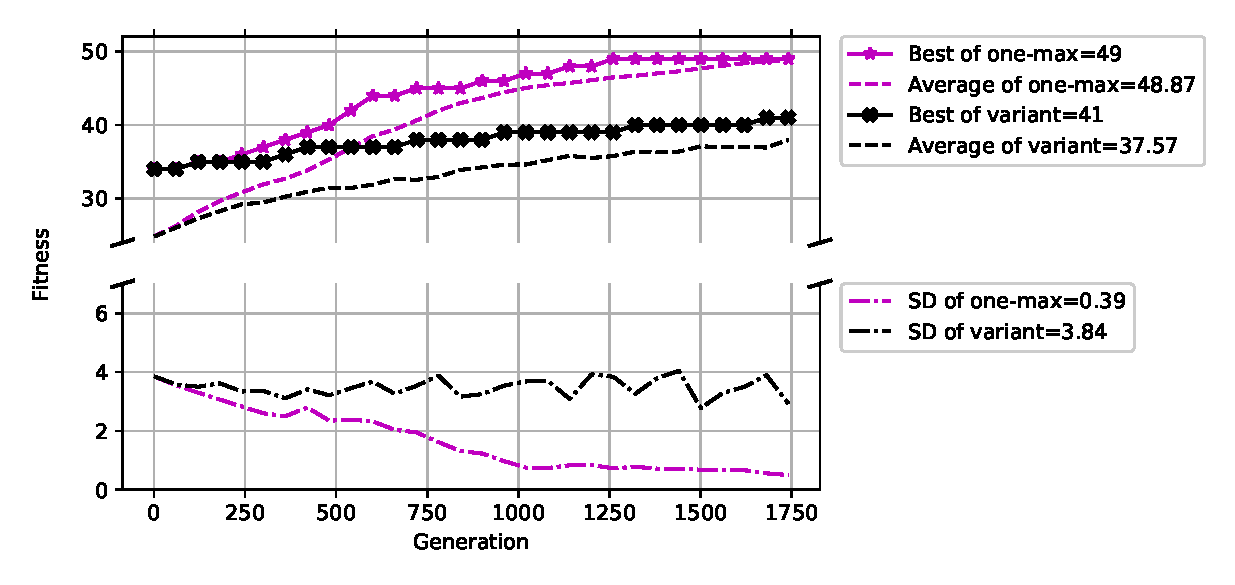
\includegraphics[width=0.45\textwidth]{body_section/figures/GECCO_onemax_vs_vonemax.eps}
  \caption{Results for the one-max and its variant with $n=50$} \label{fig:results_one_vs_vone}
\end{figure}
 

\subsubsection{Finding a Good Basis on Variant One-max Problem}
The method to consider all the bases in the one-max problem is equal to do the number of $ | GL_n (\Z_2 )| $.
The number is equal to 9,999,360 when $ n $ is 5 and the number increases exponentially as $n$ increases.
This is the case not just for the one-max problem but also for all problems related to binary representation.
It may be costly to find a good basis from all the bases.

This experiment shows that a reasonably good basis is likely to have an effect on searching for the optimal solution for genetic algorithms.
The standard basis is designed to search for the optimal solution to the one-max problem, and finds the optimal solution well.
It is not meaningful to find better ones because the standard basis is already a reasonably good basis.
A basis randomly generated in the variant one-max problem is not considered to be a good basis.
An experiment was conducted by generating the change in coordinate matrix to find a good basis as described in Section~\ref{section:ga_ccm}.
The experimental results are shown in Table~\ref{tab:results_var}.

\begin{table}[H]
  \caption{Results of our genetic algorithm for finding a good basis on the variant one-max problem}
  \label{tab:results_var}
  \begin{tabularx}{0.45\textwidth}{C{0.1\textwidth}YYY}
    \toprule
    $ n $(=optimum)    & Best & Average     &  S.D. \\
    \midrule
    $ 30  $  &  $ 27 $       &  $ 23.83 $  &  $ 1.44 $ \\
    $ 50  $  &  $ 47 $       &  $ 47.00 $  &  $ 0.00 $ \\
    $ 100 $  &  $ 99 $       &  $ 98.57 $  &  $ 2.01 $ \\
  \bottomrule
  \end{tabularx}
\end{table}

Finding a good basis is a more difficult problem than solving the variant one-max problem.
If the individual size is $ n $ for the variant one-max problem,
the $ 2^n $ solutions must be searched for,
but there needs to be the cost of $ | GL_n (\Z_2 )| \in O(2^{n^2}) $ for a good basis.
We can see that the basis search presented in Section~\ref{section:ga_ccm} is meaningful in the variant one-max problem.
When $ n $ is 100, the optimal solution of the one-max problem is found up to 99, and that of the variant one-max problem is found up to 85.
Figure~\ref{fig:cog} shows that the optimal solution on the variant one-max problem was obtained through the basis search, and that the basis search algorithm is meaningful.

\begin{figure}[H]
    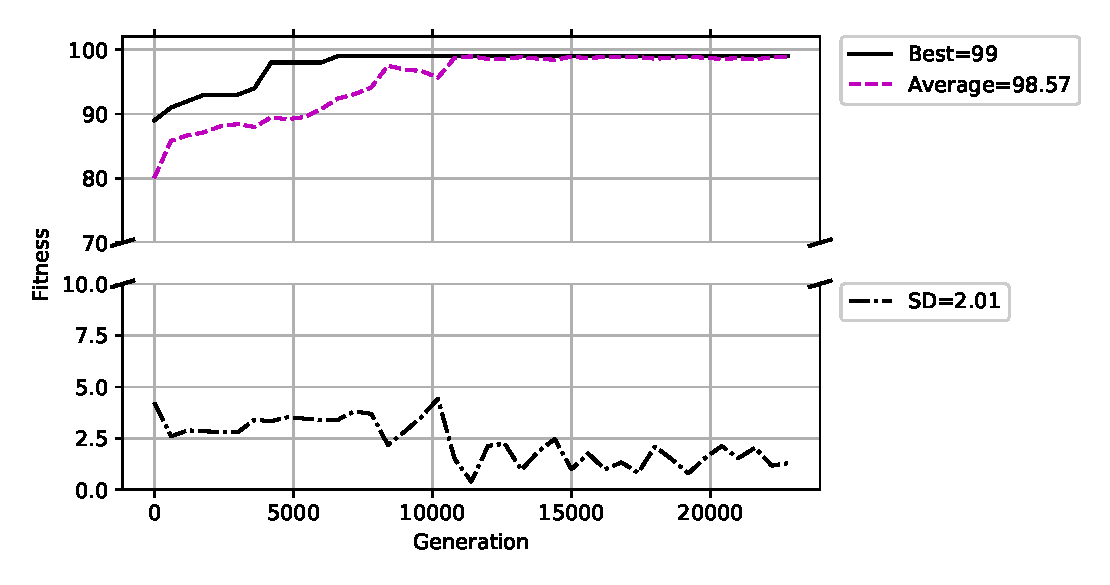
\includegraphics[width=0.45\textwidth]{body_section/figures/GECCO_cob.eps}
\caption{Results of our genetic algorithm for finding a good basis with $ n = 100 $} \label{fig:cog}
\end{figure}


\subsection{$ NK $-landscape Model}
The $NK$-landscape model consists of a string of length $N$ and fitness is contributed to each character.
In addition, the value for each character is set depending on the other $K$ characters.
These are known as fitness contributions; fitness values are set depending on one character and other $K$ characters.
These fitness contributions are often randomly chosen from a particular probability distribution.

One of the reasons why the $NK$-landscape model is used in optimization is that it is a simple instance of the NP-complete problem.
In addition, the number of hills and valleys can be adjusted through $N$ and $K$.
This experiment aims to confirm whether a good basis in binary representation is meaningful in a generally difficult problem space such as NP-complete problem,
how effective it is, and whether the basis plays an important role.

The structure of the experiment is as follows.
Initialize fitness contributions using the uniform distribution on interval $[0,1]$.
Calculate the fitness function as the average of the fitness contributed to each character.
Perform the genetic operator in the same way as on the one-max problem.
In other words, the fitness of an individual is limited to minimum of 0 and maximum of $1$.
The minimum and maximum values are unknown without inspecting every individual.
The following shows the experimental results of the $NK$-landscape model.


\begin{table}[H]
  \caption{Results for $ NK $-landscape model with $ N = 50 $ according to $ K $}
  \label{tab:results_nk_50}
  \begin{tabularx}{0.45\textwidth}{YYYY}
    \toprule
    $ K $    & Best & Average     &  S.D. \\
    \midrule
    $ 3  $  &  $ 0.72 $  &  $ 0.67 $  &  $ 0.02 $ \\
    $ 5  $  &  $ 0.70 $  &  $ 0.66 $  &  $ 0.03 $ \\
    $ 10 $  &  $ 0.70 $  &  $ 0.60 $  &  $ 0.05 $ \\
    $ 20 $  &  $ 0.66 $  &  $ 0.56 $  &  $ 0.05 $ \\
    $ 25 $  &  $ 0.62 $  &  $ 0.53 $  &  $ 0.06 $ \\
  \bottomrule
  \end{tabularx}
\end{table}

\begin{table}[H]
  \caption{Results for $ NK $-landscape model with $ N = 100 $ according to $ K $}
  \label{tab:results_nk_100}
  \begin{tabularx}{0.45\textwidth}{YYYY}
    \toprule
    $ K $    & Best & Average     &  S.D. \\
    \midrule
    $ 3  $  &  $ 0.71 $  &  $ 0.67 $  &  $ 0.02 $ \\
    $ 5  $  &  $ 0.69 $  &  $ 0.66 $  &  $ 0.02 $ \\
    $ 10 $  &  $ 0.66 $  &  $ 0.58 $  &  $ 0.04 $ \\
    $ 20 $  &  $ 0.61 $  &  $ 0.53 $  &  $ 0.04 $ \\
    $ 25 $  &  $ 0.63 $  &  $ 0.54 $  &  $ 0.04 $ \\
  \bottomrule
  \end{tabularx}
\end{table}
Tables~\ref{tab:results_nk_50} and~\ref{tab:results_nk_100} show that the generations are 1,500 and 6,000, respectively, when $ N $ is 50 and 100 in the $NK$-landscape model.
We used the same genetic operators as on the one-max problem.
The best and average fitness values tend to decrease, and standard deviations tend to increase, as $ K $ increases.
This shows that the higher the $ K $ value, the more complicated the problem of the $NK$-landscape model.

\subsubsection{Finding a Good Basis on $ NK $-landscape Model}
For the one-max problem, we can assume, to an extent, that the standard basis is a desired basis.
In fact, it is difficult to say that it is not a good basis based on the experimental results of Tables~\ref{tab:results_nk_cob_50} and~\ref{tab:results_nk_cob_100}.
Moreover, we cannot even assume what is a good basis in the $NK$-landscape model.
The problem always changes as the model for the corresponding problem is generated from a specific probability distribution.
Currently, the $NK$-landscape model can be viewed as the same as the variant one-max problem in Section~\ref{section:vonemax}
The standard basis is used as the basis of the current problem space.
However, it seems that the former genetic operators may be difficult to work properly when the problem space changes.
The following is an experiment conducted by transforming the basis from the same $ NK $-landscape model above.

\begin{table}[H]
  \caption{Results of our genetic algorithm for finding a good basis in $ NK $-landscape model with $ N = 50 $ according to $ K $}
  \label{tab:results_nk_cob_50}
  \begin{tabularx}{0.45\textwidth}{YYYY}
    \toprule
    $ K $    & Best & Average     &  S.D. \\
    \midrule
    $ 3  $  &  $ 0.77 $  &  $ 0.76 $  &  $ 0.02 $ \\
    $ 5  $  &  $ 0.78 $  &  $ 0.78 $  &  $ 0.01 $ \\
    $ 10 $  &  $ 0.77 $  &  $ 0.73 $  &  $ 0.05 $ \\
    $ 20 $  &  $ 0.74 $  &  $ 0.72 $  &  $ 0.02 $ \\
    $ 25 $  &  $ 0.73 $  &  $ 0.71 $  &  $ 0.04 $ \\
  \bottomrule
  \end{tabularx}
\end{table}

\begin{table}[H]
  \caption{Results of our genetic algorithm for finding a good basis in $ NK $-landscape model with $ N = 100 $ according to $ K $}
  \label{tab:results_nk_cob_100}
  \begin{tabularx}{0.45\textwidth}{YYYY}
    \toprule
    $ K $    & Best & Average     &  S.D. \\
    \midrule
    $ 3  $  &  $ 0.76 $  &  $ 0.75 $  &  $ 0.01 $ \\
    $ 5  $  &  $ 0.76 $  &  $ 0.76 $  &  $ 0.02 $ \\
    $ 10 $  &  $ 0.74 $  &  $ 0.73 $  &  $ 0.02 $ \\
    $ 20 $  &  $ 0.68 $  &  $ 0.68 $  &  $ 0.01 $ \\
    $ 25 $  &  $ 0.67 $  &  $ 0.67 $  &  $ 0.01 $ \\
  \bottomrule
  \end{tabularx}
\end{table}

The quality of the solution is far superior to that of the existing solution by just changing the basis in the $NK$-landscape model.
As with the variant one-max, the $NK$-landscape model uses a one-point crossover.
This genetic operator is considered to be difficult when used to find an optimal solution.
The reason is that the one-point crossover is not reflected in the problem space at all,
whereas the value of the $K+1$ element is changed in the $NK$-landscape model.
We did not implement genetic operators specific to $NK$-landscape model-specific problems.
We used a one-point crossover that is a typical crossover.
It is considered that the given operator finds a good basis that effectively finds the quality of the solution by linearly transforming the problem space through the basis.
Figure~\ref{fig:results_nk_100_10} shows that the optimal solution and the $NK$-landscape model was obtained through the basis search with $ N = 100 $ and $ K = 10 $.

\begin{figure}[H]
    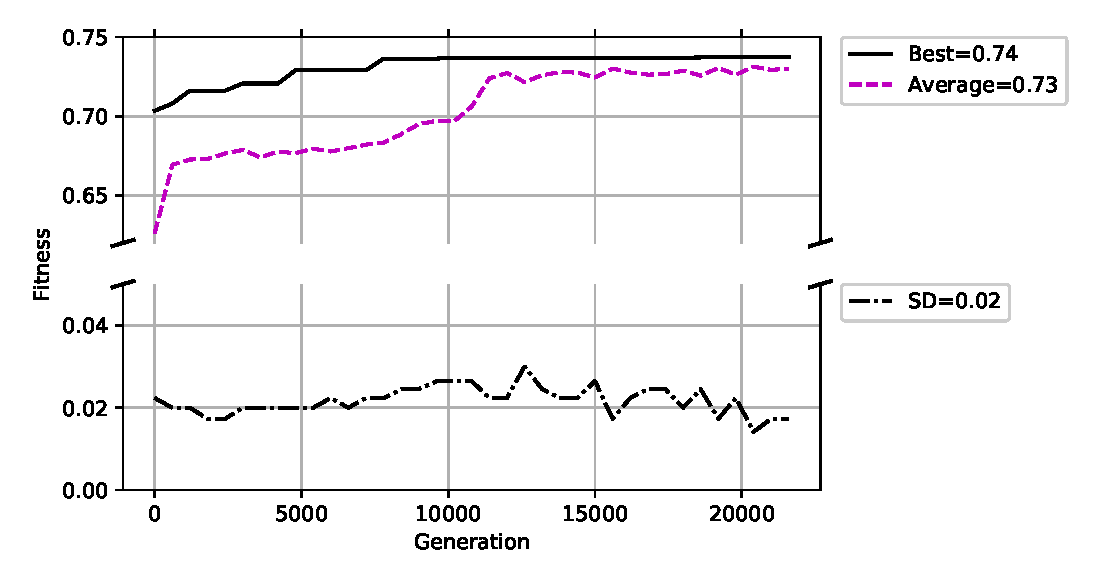
\includegraphics[width=0.45\textwidth]{body_section/figures/GECCO_cob_nk.eps}
\caption{Results of our genetic algorithm for finding a good basis on $ NK $-landscape model with $ N = 100 $ and $ K = 10 $} \label{fig:results_nk_100_10}
\end{figure}


\section{Conclusions} \label{section:conclusions}
It was not easy to determine a good basis from the one-max problem and the $NK$-landscape model; in addition, we determined how useful it was.
Currently, it is costly to find a good basis; However, if there is a good basis, it is sure to obtain a better-quality solution with the same algorithm.
Currently there are many genetic operators.
The reason is that a good quality solution will not be achieved unless appropriate genetic operators for each problem space is used.
However, there is a need for a new genetic operator to transform problem space through the basis.

Searching for a solution through a genetic algorithm to determine whether the basis is an appropriate basis of the problem space, requires a process; however, this is not practical owing to its time cost.
It may, however, be possible to practically apply a basis to a genetic algorithm if a method of heuristically evaluating the basis is devised.
For example, while we can evaluate the basis with epistasis, it is realistically impossible to obtain the value of epistasis between genes.
A good basis can therefore be obtained by estimating the basis in the direction of decreasing epistasis as the good one by using the estimate of epistasis through sampling~\cite{yu2017epistasis}.

In this study, we conducted a process to obtain the change in coordinate matrix through a genetic algorithm.
This matrix, however, can also generate instances of various levels of difficulty that have a unique solution in a light-bulb puzzle.
Furthermore, We dealt with binary encoding, but we can apply it to all $ GL_n(\mathcal{R})$  for $n$, where $\mathcal{R}$ is a commutative unital ring.



%\appendix
%Appendix A
%\section{Headings in Appendices}
%The rules about hierarchical headings discussed above for

%\begin{acks}
%\end{acks}


\bibliographystyle{bib/ACM-Reference-Format}
\bibliography{bib/sample-bibliography} 

\end{document}
